\documentclass[11pt]{exam}
\printanswers
% \documentclass[a4paper,10pt]{article}
\usepackage{tikz}
\usetikzlibrary{arrows,positioning,shapes.geometric}
\usepackage{amsmath,amssymb,complexity}
\usepackage{datetime,enumerate,palatino}
\usepackage{setspace}

\usepackage[utf8]{inputenc}
\usepackage[numbers]{natbib}
\usepackage{mathpartir}
\usepackage{mathtools}
\usepackage{mathpartir}
\usepackage{stmaryrd}
\usepackage{amsfonts}
\usepackage{amsmath}
\usepackage{amsthm}
\usepackage{listings}
\usepackage{multirow}
\usepackage[T1]{fontenc}
\usepackage{helvet}
\usepackage{array}
\usepackage{ragged2e}
\usepackage{tfrupee}  

\textwidth6in

\setlength{\topmargin}{0in} \addtolength{\topmargin}{-\headheight}
\addtolength{\topmargin}{-\headsep}

\setlength{\oddsidemargin}{0in}

\oddsidemargin  0.2in \evensidemargin 0.0in %\parindent0em


\newtheorem{theorem}{Theorem}
\newtheorem{lemma}{Lemma}
\newtheorem{corollary}{Corollary}
\newcommand\tab[1][1cm]{\hspace*{#1}}

%opening
\title{Your Name\\ Your ID}
\author{}
\date{}
\begin{document}

\hrule
\vspace{3mm}
\noindent
{\sf CS6190: Recent Developments in Theoretical Computer Science  \hfill Assignment \#1 }
\vspace{3mm}
\noindent
% {\sf Topic: OFWs and PRGs\hfill Due on : $29^{th}$ Dec, 2020}
% \vspace{3mm}
%\hrule

% uncomment the lines below and fill name and roll number of teammates here

%\vspace{3mm}
\noindent
{\sf Roll No: CS14B043\hfill Full Name: Harshal Gawai} 
\vspace{3mm}
\hrule

\begin{questions}
\question Byteland, a country of area exactly $n$ square miles, has been divided by the government into
$n$ regions, each of area exactly one square mile. Meanwhile, the army of Byteland divided
its area into $n$ military zones, each of area again exactly one square mile. Show that one can
build   $n$ airports in Byteland, such that each region and each military zone contains (at least)
one airport. Furthermore, we can find locations where we should build such $n$ airports in
polynomial time.

\begin{solution}
    Construct the following bipartite graph: on one side there are regions of Byteland, on
the second side there are military zones, and a region R is adjacent to a zone Z if R∩Z = ∅.
Show that this graph satisfies the condition of Hall’s theorem and, consequently, contains
a perfect matching.\\\\
    
    The area of Byteland is $\pmb{n}$ $mi^2$ (i.e. $n$ square miles)\\
    Which is divided into $\pmb{n}$ small areas each of $1$ $mi^2$ by government and army each in their own way.\\
    This small areas are all polygons. (i.e. $\pmb{n}$ polygons)\\
    Let \textbf{map1} and \textbf{map2} be two map schemes by government and by army respectively.\\\\

    \textbf{To prove:-} $n$ airports can be built, such that each region and each military zone contains (at least) one airport.\\
    Lets place two maps \textbf{map1} and \textbf{map2} on top of another.\\
    we are looking for airports placed common through set of polygons both maps\\
    $\therefore$ We have to prove that an airport exit common on one polygon of one sheet and another polygon of the other sheet.\\
    i.e. Each airport is common to only two polygons(one from map1 other from map2).\\
    
    Construct a bipartite graph $\pmb{G} = \pmb{R} \cup \pmb{Z}$, $\pmb{R} = \{ r_1, r_2 . ., r_n \}$ and $\pmb{Z} = \{ z_1, z_2 . ., z_n \}$ with the bipartite sets being the $\pmb{n}$ polygons in either map.\\
    
    At this point, an idea is that the edges of the matching are the airports themselves.\\
    At micro-scale of this problem consider set $\mathbb{W}$ of polygons on $\pmb{map1}$ \\
    We need to prove that there are at least $|\mathbb{W}|$ polygons on the other map $\pmb{map2}$ that touch this subset $\mathbb{W}$.\\
    \\
    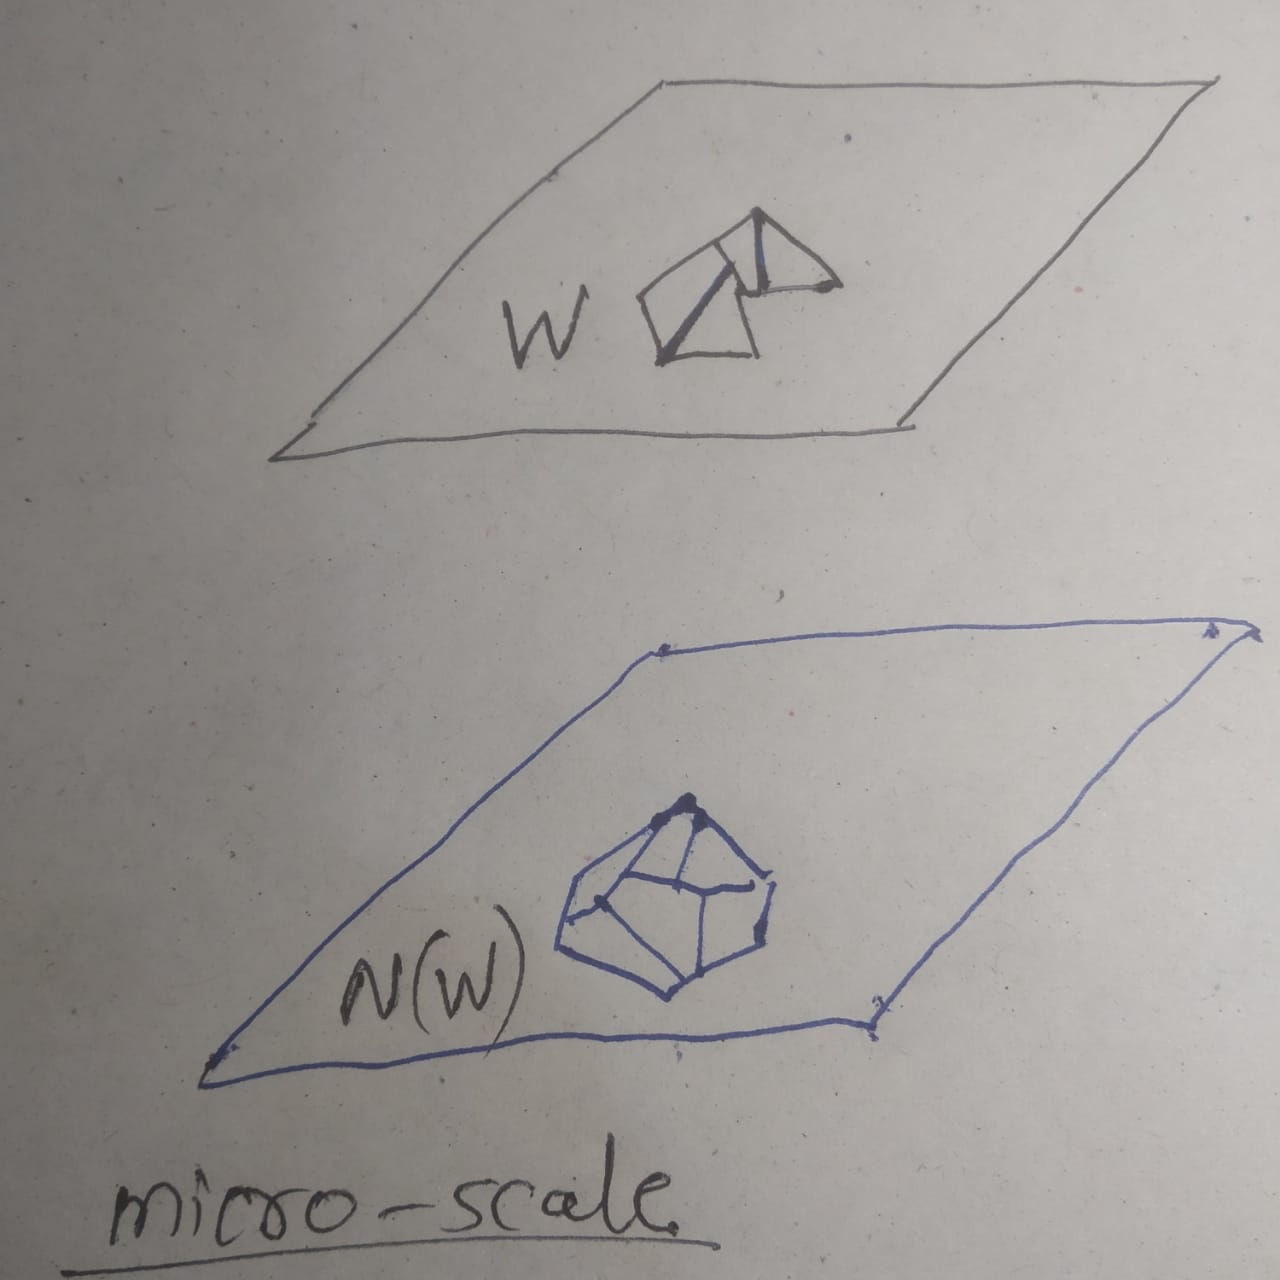
\includegraphics[scale=0.15]{fig1.jpeg} 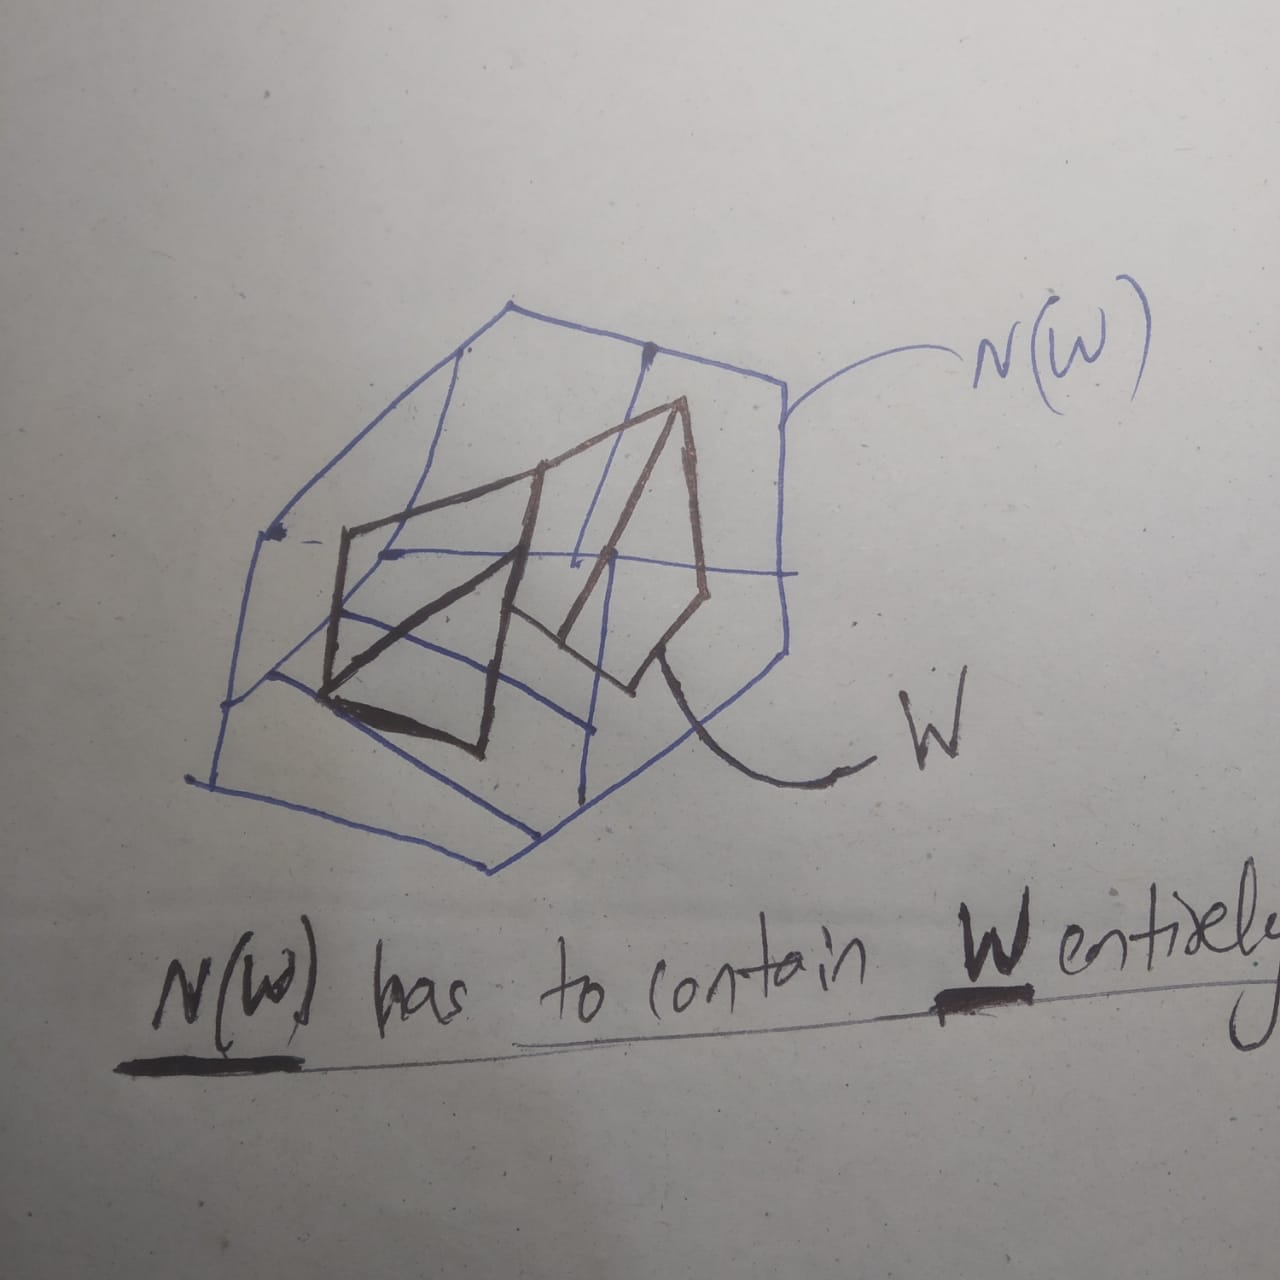
\includegraphics[scale=0.15]{fig2.jpeg}
    \\
    We try contradiction\\
    
    Take $\mathbb{W}$ and suppose that, say, less than $|\mathbb{W}|$ polygons intersect with it on the other map.\\
    We write $N(\mathbb{W})$ to denote the neighborhood of a set $\mathbb{W}$: the set of all vertices adjacent to some vertex of $\mathbb{W}$.\\
    i.e. assume $N(\mathbb{W}) < \mathbb{W}$\\
    Intuitively, this must mean that the polygons of $\mathbb{W}$ are “smaller” than those on $N(\mathbb{W})$, because they both occupy the same area\\
    We haven't used the information that each polygon have an area of $1$ $mi^2$\\\\
    $\implies$  The polygons of $\mathbb{W}$ have an area of exactly $|\mathbb{W}|$\\
    And the polygons of $N(\mathbb{W})$ have an area of exactly $|N(\mathbb{W})|$.\\
    But the region $N(\mathbb{W})$ has to contain the region of $\mathbb{W}$\\
    $\implies   \mathbb{W} \leq N(\mathbb{W})$ for any subset $\mathbb{W}$\\
    
    $\therefore$ by Hall’s theorem there exists a matching from one set of polygons to the other. We use this matching to find appropriate positions for the airports.
    
    
    
    
    
\end{solution}

%%%%%%%%%            %%%%%%%%%%%%            %%%%%%%%%%%           %%%%%%%%%%%%%           %%%%%%%%%%%%
\question Show that any graph has at most $2^k$ inclusion-wise minimal vertex covers of size at most
$k$. Furthermore, show that given $\pmb{G}$ and an integer $k$, we can enumerate all inclusion-wise
minimal vertex covers of $\pmb{G}$ of size at most $k$ in time $2^k|V(\pmb{G})|)^{O(1)}$ .
\begin{solution}
    3.3 Consider the following branching algorithm: given an instance (G, k), pick an arbitrary
edge uv ∈ E(G) and branch on two instances (G − u, k − 1) and (G − v, k − 1). Stop when
G becomes edgeless or k < 0. Show that in this manner you generate at most 2 k leaves
of the search tree, and every minimal vertex cover of G of size at most k appears in some
leaf.
\end{solution}

%%%%%%%%%            %%%%%%%%%%%%            %%%%%%%%%%%           %%%%%%%%%%%%%           %%%%%%%%%%%%
\question In the \textsc{Cluster Vertex Deletion} problem, we are given a graph $\pmb{G}$ and an integer $k$, and the
task is to delete at most $k$ vertices from $\pmb{G}$ to obtain a cluster graph (a disjoint union of cliques).
    Obtain a $3^k|V(\pmb{G})|^{O(1)}$ -time algorithm for \textsc{Cluster Vertex Deletion}.
\begin{solution}
    4.5 The exercise boils down to a task of showing that the disjoint version of the problem
is polynomial-time solvable.
First, observe that a graph is a cluster graph if and only if it does not have an induced
path on three vertices. In the disjoint version of the problem, given (G, S, k) such that
|S| = k + 1 and G − S is a cluster graph, we are looking for a solution of size at most k
such that it is disjoint from S.
• We can assume that the subgraph induced on S is a cluster graph. Why?
• What can you do if there is a vertex in V (G) \ S that is adjacent to two of the clusters
of G[S], the subgraph induced on S? Or a vertex in V (G) \ S that is adjacent to some,
but not all vertices of one of the clusters of G[S]?
• Now we can assume that every vertex in V (G)\S is either completely nonadjacent to S,
or completely adjacent to exactly one cluster of G[S]. Argue that the resulting problem
(of finding a subset of vertices to be deleted from V (G) \ S to make the resulting graph
a cluster graph) can be solved by using an algorithm for finding a maximum matching
of minimum cost in a bipartite graph.
\end{solution}

%%%%%%%%%            %%%%%%%%%%%%            %%%%%%%%%%%           %%%%%%%%%%%%%           %%%%%%%%%%%%
\question Prove that for a tournament $\pmb{T}$ , the following properties are satisfied:\\
1. $\pmb{T}$ has a directed cycle if and only if $\pmb{T}$ has a directed triangle;\\
2. If $\pmb{T}$ has no directed cycle, then it has unique topological ordering. That is, there exists a unique ordering $<$ of the vertices of $\pmb{T}$ such that for every directed edge $(u, v)$ , we have
$u < v$ (that is, $u$ appears before $v$ in the ordering $<$ ).
\begin{solution}
    4.2.1 Solving Disjoint Feedback Vertex Set in Tournaments in polynomial time\\
    Lemma 4.3. Let
\end{solution}

%%%%%%%%%            %%%%%%%%%%%%            %%%%%%%%%%%           %%%%%%%%%%%%%           %%%%%%%%%%%%
\question A graph $\pmb{G}$ is a \emph{split graph} if $V(\pmb{G})$ can be partitioned into sets $\mathbb{C}$ and $\mathbb{I}$ such that $\mathbb{C}$ is a clique and $\mathbb{I}$ is an independent set in $\pmb{G}$. In the \textsc{Split Vertex Deletion} problem, given a graph $\pmb{G}$ and an integer $k$, the task is to check if one can delete at most $k$ vertices from $\pmb{G}$ to obtain a split graph.\\\\
Design a $2^k|V(G)|^{O(1)}$ algorithm for \textsc{Split Vertex Deletion}, using iterative compression.
\begin{solution}

    4.6 Again, the task reduces to showing that the disjoint version of the problem is
polynomial-time solvable.
The main observation is that a split graph on n vertices has at most n 2 partitions of
the vertex set into the clique and independent set part: for a fixed one partition, at most
one vertex can be moved from the clique side to the independent one, and at most one
vertex can be moved in the opposite direction. (In fact one can show that it has at most
O(n) split partitions.) Hence, you can afford guessing the “co
\end{solution}

%%%%%%%%%            %%%%%%%%%%%%            %%%%%%%%%%%           %%%%%%%%%%%%%           %%%%%%%%%%%%
\question In \textsc{Triangle Packing} problem, we are given a graph $\pmb{G}$ and an integer $k$, and the objective is to test whether $\pmb{G}$ has $k$-vertex disjoint triangles. Design a (deterministic) algorithm for the problem running in time $2^{O(k)}|V(G)|^{O(1)}$ .
\begin{solution}

\end{solution}

%%%%%%%%%            %%%%%%%%%%%%            %%%%%%%%%%%           %%%%%%%%%%%%%           %%%%%%%%%%%%
\question In the \textsc{Cycle}/\textsubscript{vc} problem, we are given a graph $\pmb{G}$, a vertex cover $\pmb{X}$ of $\pmb{G}$ of size $k$, and an integer $l$ , and the objective is to test if $\pmb{G}$ has a cycle on at least $l$ vertices.\\\\
Design an FPT algorithm for \textsc{Cycle}/\textsubscript{vc}, when parameterized by $k$ (the size of the given vertex cover).
\begin{solution}

\end{solution}


\end{questions}
\end{document}
